\section{LSTM model}
In this section we present the experimental results based on research studies on BitBrain data set. 
For training a model BitBrain Rnd dataset is very useful. Dataset has 3 month trace of 5 min of interval. More than 12 million dataset of 5 min of interval trace resample into hourly based to predict the future resoruce usage on VM. From dataset 75% data used as training data and other 25% used as testing data. Once data is stored into datframe then first remove Nan value from the dataset. For deep learning model it requires to convert data into range between 0 to 1. Normalization require since all the model perform complex calculation, after getting result create input data and labels  for the model. Input data is previous lags of current timestamp, if you select 10 lag value then 10 previous value of  current timestamp consider as input data and current timestamp as label for particular input data.
\begin{figure}
  \centering
    
      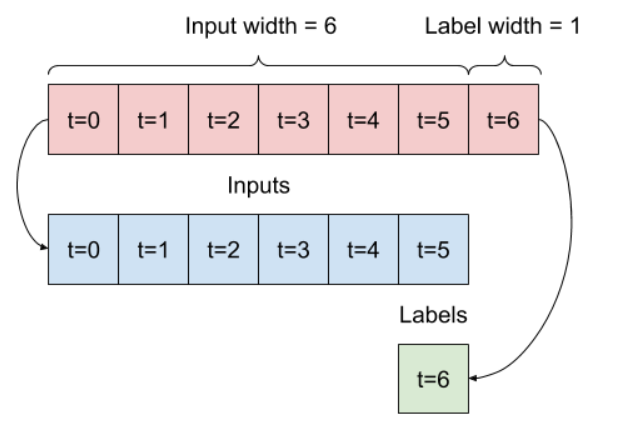
\includegraphics[width=1\textwidth]{tensorflow.png}
  \caption{lag order plot based on AIC score}
  \label{fig:nn}
\end{figure}
Figure \ref{fig:nn} mentioned how to predict 1-hour data based on previous 6h information where previous 6h data classified as input data for current timestamp data. After convert input data and labels it is important that data must be in (samples, timestamp, feature) format.Reshape dataset and pass the information to the all sequential model. For experimental analysis dataset pass to four model first vanilla LSTM, multi hidden layer LSTM, first Bi-LSTM, and multi-hidden layer LSTM.


\begin{figure}[htp]

\subfloat[Vanilla LSTM]{
  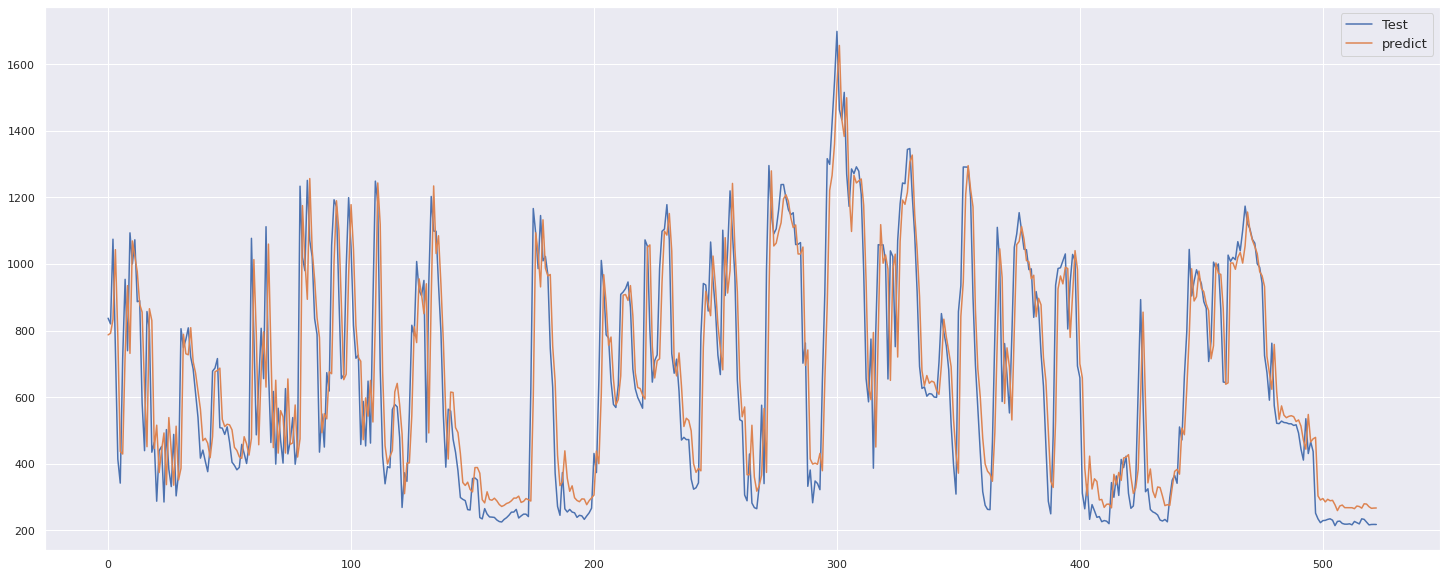
\includegraphics[width=1\linewidth,height=5cm]{model1.png}%
}

\subfloat[Vanilla LSTM model with lambda layer]{
  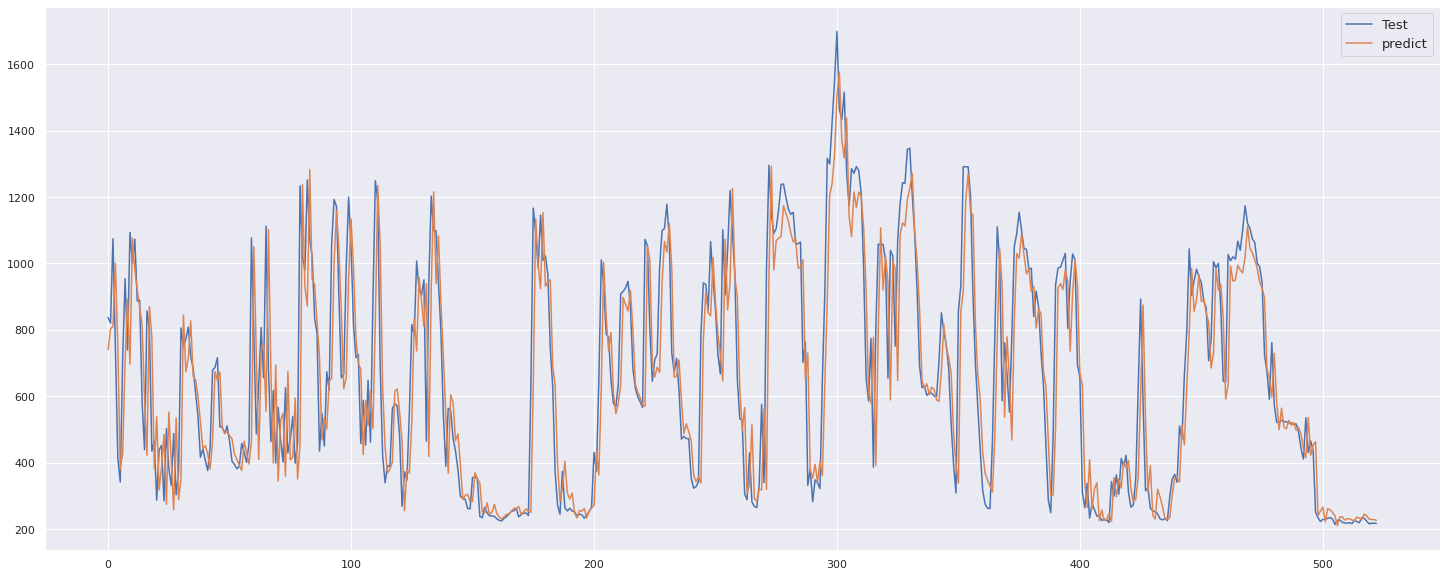
\includegraphics[width=1\linewidth,height=5cm]{lambdamodel2.png}%
}

\subfloat[Multilayer of LSTM model]{
  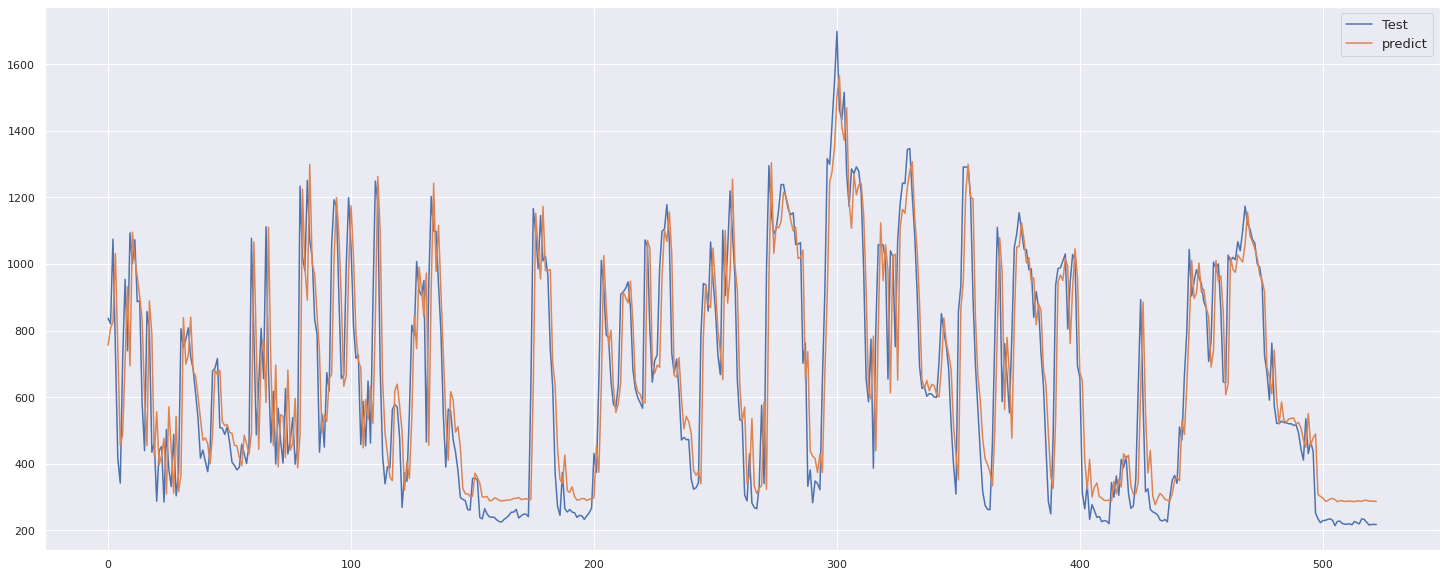
\includegraphics[width=1\linewidth,height=5cm]{lstmmodel3.png}%
}
\caption{test vs prediction of data on LSTM Model }
\label{fig:vanilla}
\end{figure}
All the vanilla models use 90 units for LSTM  layers with ReLU activation function after that use the dropout layer to prevent overfitting problems, then add a dense layer to the model. After creating a model compile model in which we use adam optimizer and also fetch accuracy and make metrics for the model. For training a model we used 32 batch sizes with 500 epochs in every Vanilla-based LSTM and Bi-LSTM model. Multiple hidden layers of LSTM and LSTM use 3 hidden layers with 90 units for each LSTM layer. The model uses ReLU activation with a 0.3 value dropout layer to prevent overfitting problems. Both models use adam optimizer with accuracy and MAE metrics, also use 32 batch size with 500 epochs to train a model.

Figure \ref{fig:vanilla} describes information about performance on a variant of the LSTM model. Figure \ref{fig:vanilla}(A) describes the Vanilla LSTM model, after training a model its generates 158.26 RMSE and 105.10 MAE error on training data while 166.83 RMSE and 119.42 MAE error on testing data. Figure \ref{fig:vanilla}(B) describes the LSTM model with the Lambda layer which uses $x=x*100$ comparison of data of the dense layer. It produces 158.55 RMSE and 101.81 MAE errors on training data while 167.74 RMSE and 114.95 MAE errors on testing data. Figure \ref{fig:vanilla}(c) describes multiple layers of the LSTM  model with 156.52 52 RMSE error and 102.83 MAE error on train data for testing data it generates 168.12 RMSE and 121.01 MAE error. Figure \ref{fig:vanillaloss} describes a comparison of training loss with validation loss by each epoch while training a model


\begin{figure}[htp]

\subfloat[Vanilla LSTM ]{
  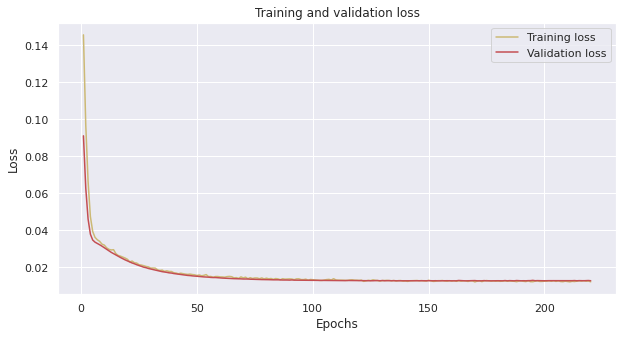
\includegraphics[width=0.5\linewidth,height=5cm]{model1loss.png}%
}
\qquad
\subfloat[Vanilla LSTM model with lambda layer]{
  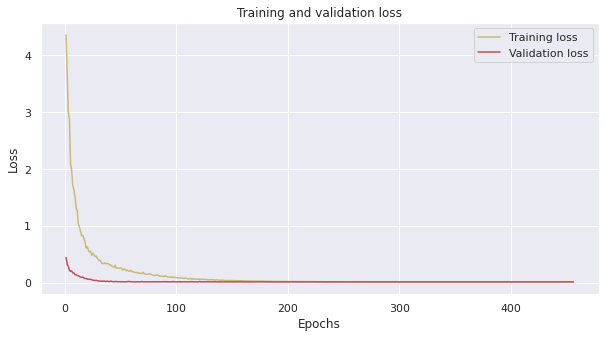
\includegraphics[width=0.5\linewidth,height=5cm]{model2loss.png}%

}
\center
\subfloat[Multilayer of LSTM model]{
  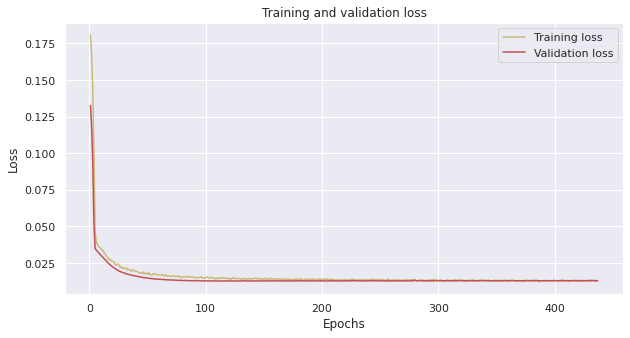
\includegraphics[width=0.5\linewidth,height=5cm]{model3loss.png}%
}
\caption{loss of  the model }
\label{fig:vanillaloss}
\end{figure}
\section{BI-LSTM model}

Figure \ref{fig:Bilstem} describe different Bi-LSTM model with single and multiple layers of Bi-LSTM. Figure \ref{fig:Bilstem} (a) describe the single layer of Bi-LSTM which produce 154.22 RMSE and 101.35 MAE.Error while training a model and 166.16 RMSE and 119.59 MAE errors while testing data applied on the model. It produces good prediction when CPU Usage to low but there is a spike in CPU usage then the prediction is not accurate to forecast the future workload. figure \ref{fig:Bilstem} (b) produces Multilayer Bi-directional LSTM on the CPU usage dataset. there is an improvement in error while training a model, it has 143.23 RMSE and 93. 49 MAE while multilayer Bi-LSTM does not produce an accurate prediction on testing data, it has 170.76 RMSE and 123.23 MAE errors. Multiple layers of Bi-LSTM produce the best prediction when there is a spike in CPU usage but do not produce an accurate result when CPU usage is very low. Figure \ref{fig:Bilstemloss} describe training loss and validation loss based on the epoch of both Bi-LSTM model.
\begin{figure}[htp]

\subfloat[single layer Bi-LSTM]{
  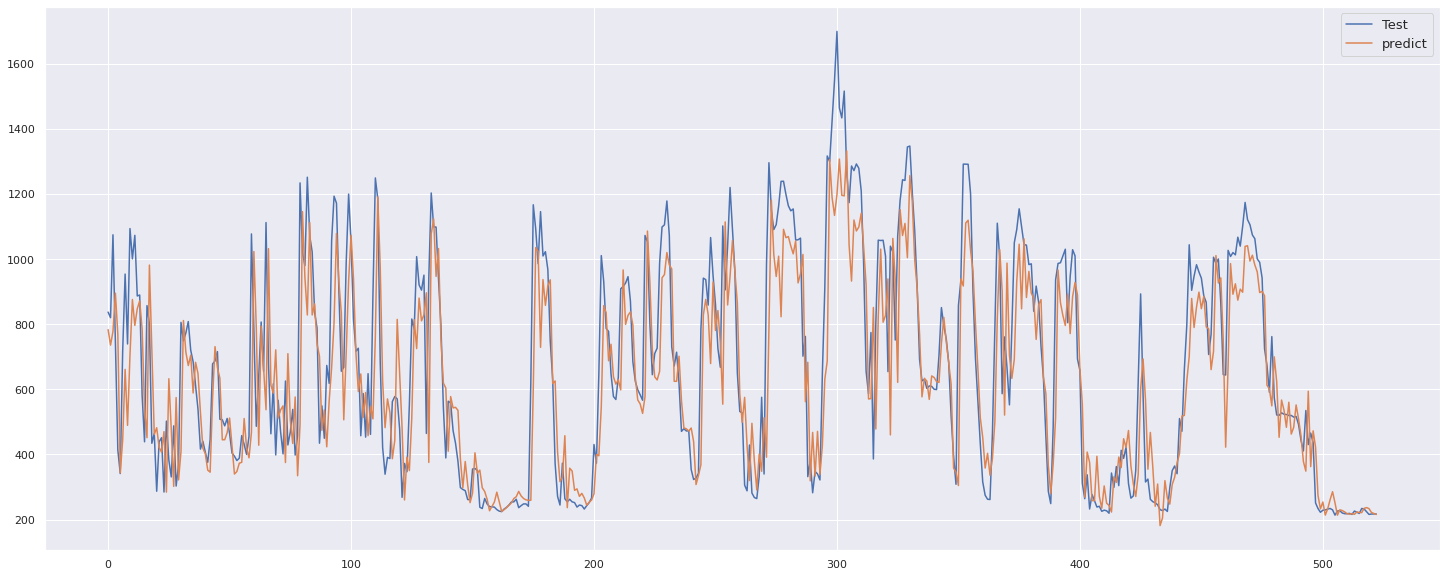
\includegraphics[width=1\linewidth,height=5cm]{Bi_LSTM single.png}%
}

\subfloat[multilayer Bi-LSTM model]{
  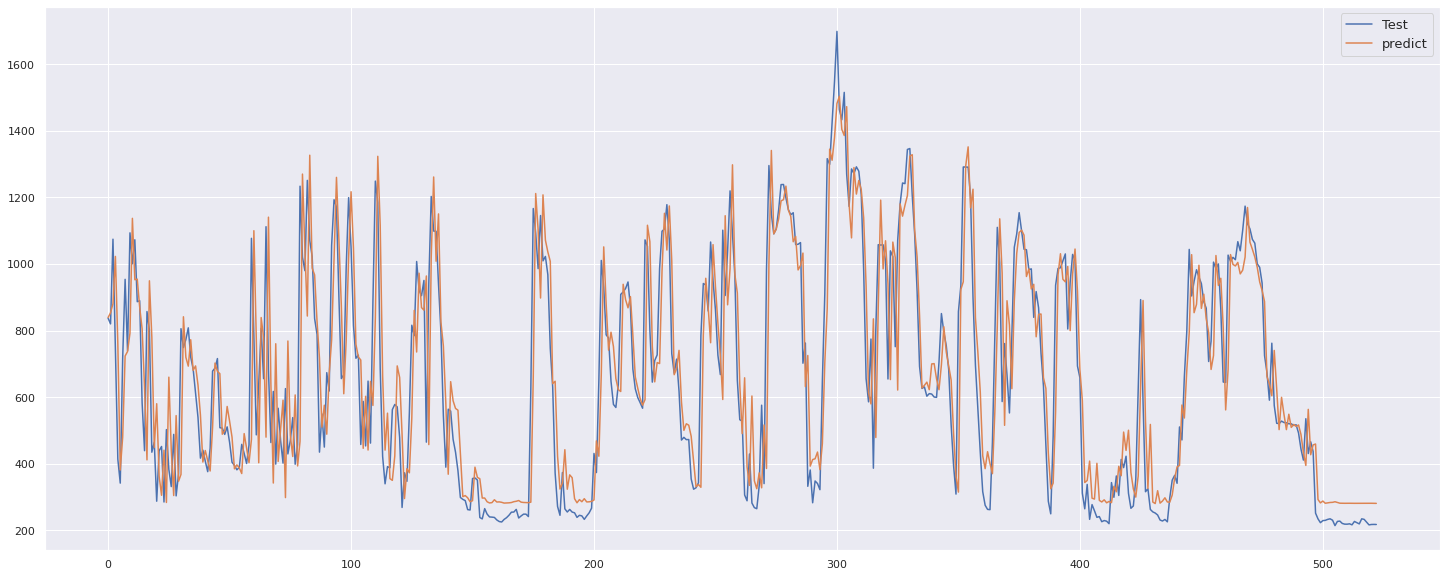
\includegraphics[width=1\linewidth,height=5cm]{Bi-LSTM.png}%
}


\caption{test vs prediction of data on Bi-LSTM Model }
\label{fig:Bilstem}
\end{figure}
All the models use the early stopping method,  early stopping is a method that uses to prevent overfitting the training model. Early stopping stops the training model on a large epoch if the performance of the model stops improving on validation observations \cite{guan2019predicting}.Table \ref{tab:score} compare all deep learning model on training and testing data while applying model on a training data Multilayer LSTM produce efficient while applying same model on a testing data Single Bi-LSTM is effective one.  result  Other performance metrics applied on all models which are mentioned above and for all the predictions refer to Appendix A.
\begin{figure}[htp]

\subfloat[single layer Bi-LSTM]{
  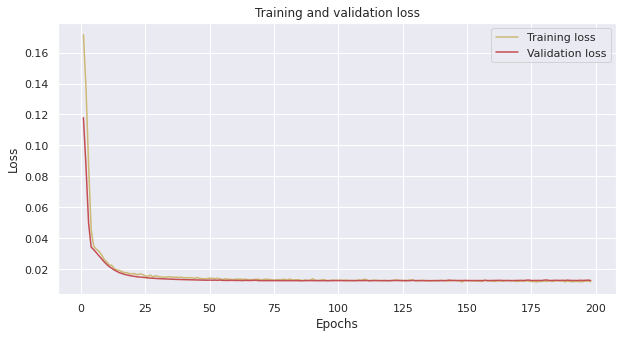
\includegraphics[width=1\linewidth,height=5cm]{model4loss.png}%
}

\subfloat[multilayer Bi-LSTM model]{
  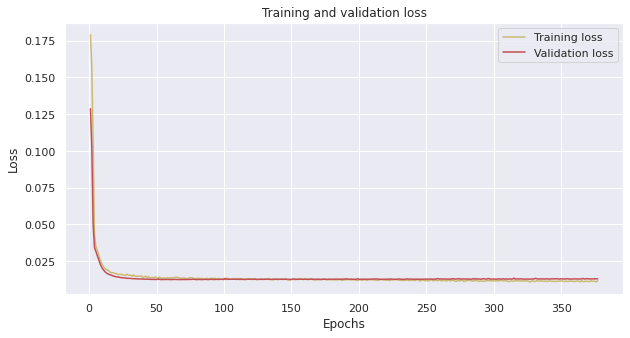
\includegraphics[width=1\linewidth,height=5cm]{model5loss.png}%
}


\caption{loss of  the model }
\label{fig:Bilstemloss}
\end{figure}

\begin{table}
\center
\caption{comparative analysis of training and testing error with Deep Learning model }
  \begin{tabular}{|l|l|l|l|l|}
    \hline
\hline
    \multirow{2}{*}{model} &
      \multicolumn{2}{c}{train} &
      \multicolumn{2}{c|}{test} \\ \cline{2-5}

    & RMSE& MAE & RMSE & MSE \\
    \hline
    Vanilla LSTM &158.26 & 105.10 & 166.83 & 119.42 \\
    \hline
    LSTM with Lambda Layer & 158.55 & 101.81& 167.74 & 114.95 \\
    \hline
    Multilayer LSTM & 156.52 & 102.83 & 168.12 & 121.01 \\
    \hline
Single Bi-LSTM &154.22&101.35&166.16&1119.59 \\
\hline
MultiLayer LSTM & 143.23&93.49 &170.76 & 125.25\\
\hline\hline
\end{tabular}
\label{tab:score}
\end{table}